\chapter{Data acquisition and processing}
\label{ch:data-acquisition}

This chapter covers the sensor suite, the laboratory calibration that traces each channel to a known physical reference and the two-stage noise-rejection pipeline that filters raw readings before they reach storage.

\section{Sensor suite}

The platform combines three numeric measurement domains with one visual observation path:
\begin{itemize}
    \item \textbf{Air conditions}: The SHT35 sensor measures air temperature and relative humidity via the I$^2$C bus \parencite{seeed-sht35}. Its $\pm$1.5\% relative humidity (RH) and $\pm$0.1$^\circ$C accuracy \parencite{sensirion-sht35} is the technical foundation for the system's VPD calculations \parencite{massmann2019vpd}. 
    \item \textbf{Light spectrum}: The TCS3448 (Color 21 Click \parencite{mikroe-color-21}) reads light on 14 separate channels. It has eight narrow-band filters (F1--F8), three broad "Commission Internationale de l'Éclairage" (CIE) XYZ-type channels (FZ$\,\leftrightarrow\,$Z tristimulus, FY$\,\leftrightarrow\,$Y/luminance, FXL$\,\leftrightarrow\,$X-long wavelength), a Near-Infrared (NIR) channel, a clear broadband visible channel (\texttt{2x\_vis\_1}) and a Flicker Detection (FD) channel that picks apart the frequency of artificial light. Where an ordinary RGB sensor collapses everything into three bands, these 14 channels are enough to reconstruct a spectral power distribution.
    \item \textbf{Plant mass}: A load cell wired to an HX711 24-bit analog-to-digital converter (ADC) \parencite{sparkfun-hx711} tracks mass. Those 24 bits are what let the station pick up the sub-gram swings evapotranspiration produces in a small potted plant.
    \item \textbf{Visual observation}: A Raspberry Pi Camera Module (v1.3, 5\,MP) takes images at fixed intervals, while a dedicated vision service handles focus, exposure and storage. I kept the v1.3 for cost and availability. Its fixed-focus lens resolves leaf area well enough at the short working distances inside this enclosure.
\end{itemize}

Every sensor sits behind the same (\texttt{BaseSensor}) interface. The hardware is shown in Figure~\ref{fig:sensor-photos}. They all share the same lifecycle. First, an initialization phase (\texttt{setup()}), then a data-retrieval phase (\texttt{read\_data()}). These are what lets the main loop treat all of the sensors as interchangeable data producers. A failed read returns a structured error payload rather than raising an exception. This makes it so in the case of one bad component, it doesn't bring down the whole acquisition loop.

\begin{figure}[H]
    \centering
    \begin{subfigure}[b]{0.32\textwidth}
        \centering
        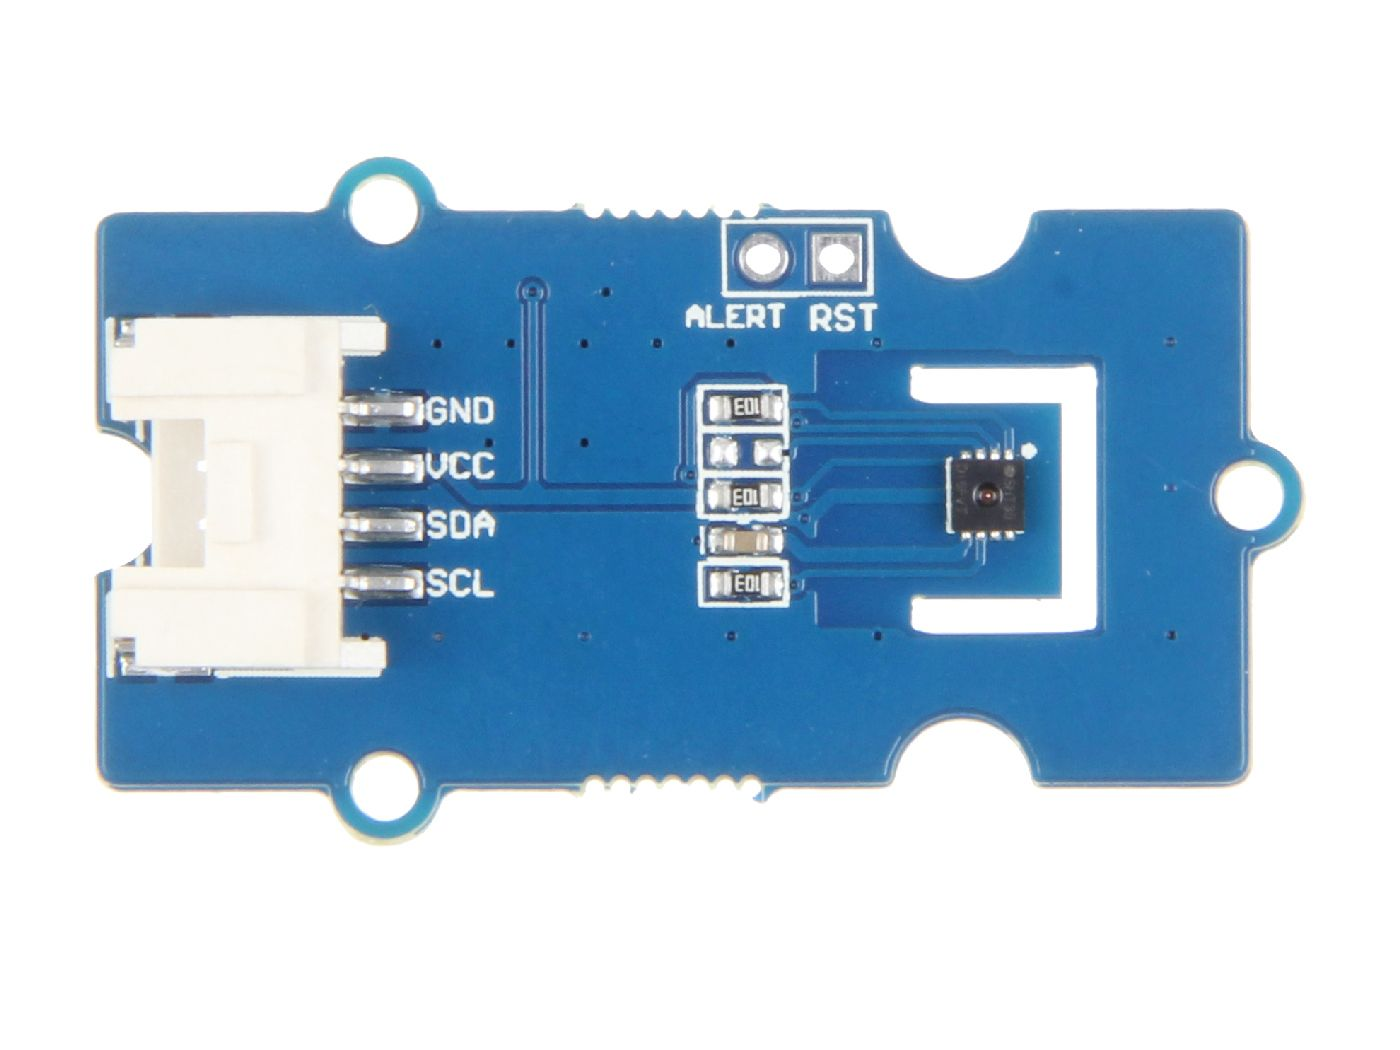
\includegraphics[width=\textwidth]{Images/sht35}
        \caption{SHT35 (Air conditions).}
        \label{fig:photo-sht35}
    \end{subfigure}
    \hfill
    \begin{subfigure}[b]{0.32\textwidth}
        \centering
        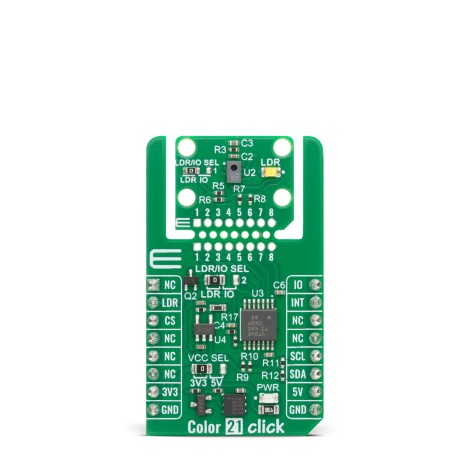
\includegraphics[width=\textwidth]{Images/tcs3448}
        \caption{TCS3448 (Light spectrum).}
        \label{fig:photo-tcs3448}
    \end{subfigure}
    \hfill
    \begin{subfigure}[b]{0.32\textwidth}
        \centering
        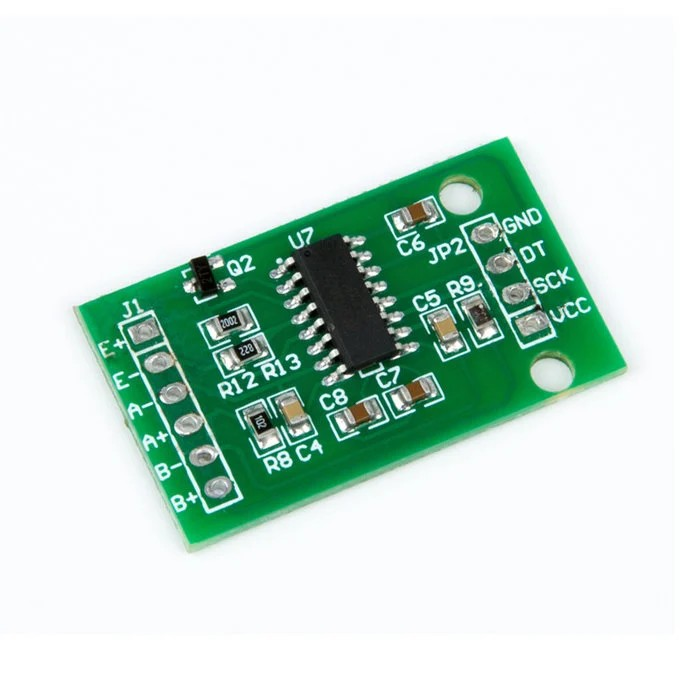
\includegraphics[width=\textwidth]{Images/hx711}
        \caption{HX711 (Plant mass).}
        \label{fig:photo-hx711}
    \end{subfigure}
    \caption[PhenoHive Core Sensor Suite]{The core numeric sensor suite of the PhenoHive station which were all selected for research-grade precision in an educational context.}
    \label{fig:sensor-photos}
\end{figure}
\section{Sensor calibration and metrological validation}

A raw sensor reading is of no use for phenotyping until it can be checked, trusted, and traced back to a known physical reference. In the context of an educational platform, this is particularly important because students need to be able to trust the data enough to reason about plant physiology and work with the collected data.Also, TAs need to be able to reproduce or check the calibration without any special expertise. The workflow I built answers both of these requirements by cross-referencing each sensor against traceable laboratory instruments at the WELCOME (Wallonia Electronics and Communications Measurements) lab \parencite{welcome-lab} and writing the resulting corrections straight into the station configuration.

\subsection{Calibration methodology}

The calibration procedure was done manually by using a steady-state reference sweep (Figure~\ref{fig:calibration-architecture}). The target conditions were adjusted directly on the reference laboratory instruments (the ESPEC climatic chamber and the monochromator combined with the optical setup) for each measurement setpoint. Once a stable and steady-state condition was reached, the reference values were recorded. 
At the same time, the raw readings from the studied sensor of the PhenoHive station was retrieved. By combining these reference measurements with the raw sensor outputs for each setpoint, a dataset was produced from which the calibration offsets and scaling factors were calculated. These offsets and scaling factors were then applied as correction values in the station's config file. This process ensured that each sensor's output was grounded in a known physical reference, allowing for accurate and reliable data collection during phenotyping experiments. 

\begin{figure}[H]
\centering
\begin{tikzpicture}[
    node distance=1.0cm and 1.8cm,
    block/.style={draw, rounded corners, align=center, text width=3.2cm, minimum height=1cm, fill=white, font=\footnotesize},
    arrow/.style={-{Latex[length=2.5mm]}, thick}
]
\node[block, fill=blue!8] (op) {TA\\(Manual Control)};
\node[block, fill=orange!8, right=of op] (eq) {Lab Equipment\\(SH242 / CM110 / Power Meter)};
\node[block, fill=green!8, below=1.5cm of op] (rpi) {PhenoHive RPi\\(Status API / Debug UI)};
\node[block, fill=gray!8, below=1.5cm of eq] (txt) {Calibration Logs\\(Reference vs.\ Sensor)};

\draw[arrow] (op) -- (eq) node[midway, above, font=\scriptsize] {Set setpoint};
\draw[arrow] (eq) -- (op) node[midway, below, font=\scriptsize] {Stabilize};
\draw[arrow] (op) -- (rpi) node[midway, left, font=\scriptsize] {Read raw values};
\draw[arrow] (op) -- (txt) node[midway, above, font=\scriptsize, sloped] {Log pair (ref\,+\,raw)};
\end{tikzpicture}
\caption[Manual Calibration Workflow]{Manual calibration workflow. Each setpoint was manually set on the reference equipment after which the raw sensor values were read after stabilization from the RPi API. Each logged calibration pair combines both the  reference instrument reading with the corresponding raw sensor output in orderto create the calibration dataset.}
\label{fig:calibration-architecture}
\end{figure}

Throughout the manual calibration the RPi kept on running as it normally would and was not put into a special calibration mode. This shows that the collected data is representative of the actual working conditions of the station.

In order to assist with the data collection, some lightweight Python scripts were used to continuously query the RPi's API. By comparing the live, raw outputs of the sensors against the stabilized laboratory equipment displays, the offsets and scaling factors were then calculated and written to the station's configuration file. 

\subsection{Environmental sensor calibration}
\label{sec:sht35-calibration}

The SHT35 temperature and humidity sensor was calibrated against an Espec SH-242 climatic chamber \parencite{espec-sh-242} which is a reference-grade instrument with active temperature and humidity regulation and factory-stated setpoint accuracies of $\pm0.3\,^\circ$C and $\pm3.0\,\%$\,RH (Figure \ref{fig:espec-sh242}). These reference accuracies set a floor on what this sweep can actually resolve. The SH-242's setpoint tolerances ($\pm0.3\,^\circ$C, $\pm3.0\,\%$\,RH) are in fact coarser than the SHT35's own datasheet accuracy ($\pm0.1\,^\circ$C, $\pm1.5\,\%$\,RH), so the exercise is best understood as a \emph{verification that the factory calibration still holds} rather than as a correction that improves on it: a chamber cannot certify a sensor to a tighter bound than its own uncertainty. The measured mean deviations ($+0.14\,^\circ$C, $-1.53\,\%$\,RH) are smaller in magnitude than the chamber's setpoint tolerance, which is the expected outcome of a sensor that agrees with the reference to within the reference's own uncertainty. The calibration followed a four-point corner sweep made to cover the extremes of the typical operating range. Two temperature levels (20$^\circ$C and 40$^\circ$C) were crossed-referenced with two humidity levels (40\% and $\approx$80\% RH). The chamber stabilized at 83\% RH rather than exactly 80\% at the 20$^\circ$C/high-humidity setpoint which is why that condition is reported as 83\% in the results. This choice of setpoints spans a bit more than the typical range for indoor plant experiments and captures both the offset and any temperature dependent drift in the humidity reading.

\begin{figure}[H]
    \centering
    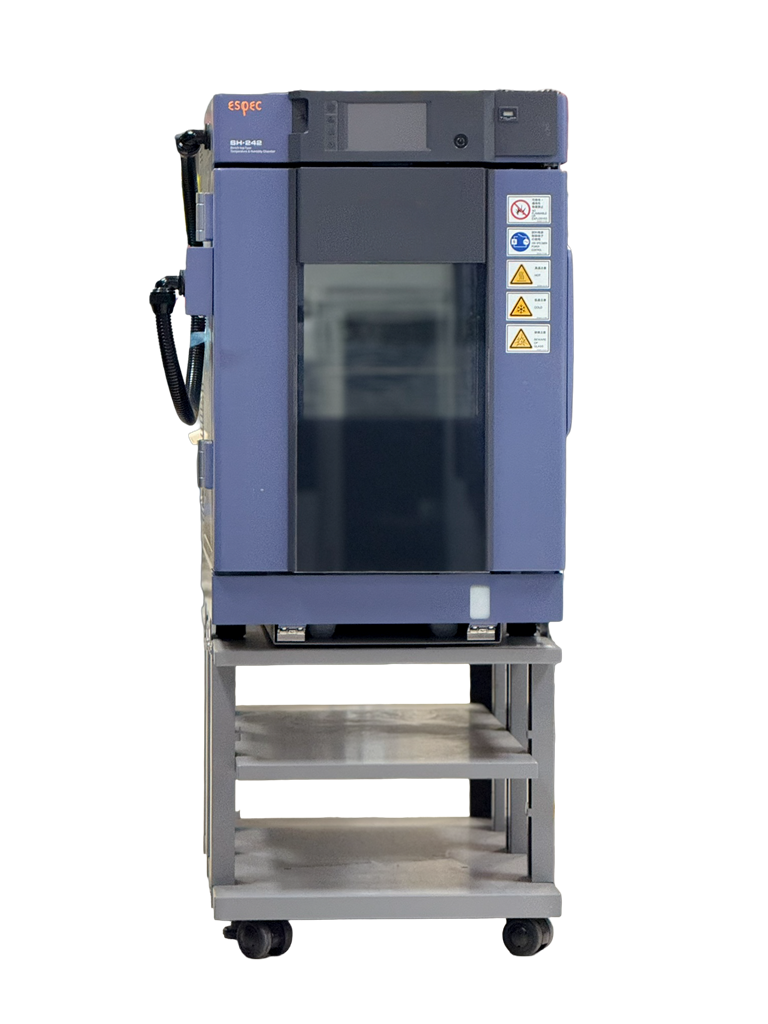
\includegraphics[width=0.5\textwidth]{Images/espec_sh242}
    \caption[Espec SH-242 Environmental Chamber]{The Espec SH-242 used for temperature and humidity sensor validation \parencite{espec-sh-242}.}
    \label{fig:espec-sh242}
\end{figure}

For each setpoint, the chamber was left for 15 minutes before the measurement was made in order for it to stabilize. 

\begin{table}[H]
\centering
\caption[SHT35 Calibration Results]{SHT35 calibration results against the SH242 climatic chamber. Each row corresponds to one stabilized setpoint. The error columns show the difference between the sensor reading and the chamber reference.}
\label{tab:sht35-calibration}
\small
\setlength{\tabcolsep}{5pt}
\renewcommand{\arraystretch}{1.25}
\begin{tabularx}{\textwidth}{|P{2.2cm}|X|X|X|X|}
\hline
\textbf{Setpoint} & \textbf{Ref.\ T ($^\circ$C)} & \textbf{SHT35 T ($^\circ$C)} & \textbf{Ref.\ RH (\%)} & \textbf{SHT35 RH (\%)} \\
\hline
20$^\circ$C / 40\% & 20.0 & 19.82 ($-$0.18) & 40.0 & 43.67 ($+$3.67) \\
\hline
20$^\circ$C / 83\% & 20.0 & 19.71 ($-$0.29) & 83.0 & 80.70 ($-$2.30) \\
\hline
40$^\circ$C / 40\% & 40.0 & 39.82 ($-$0.18) & 40.0 & 42.66 ($+$2.66) \\
\hline
40$^\circ$C / 80\% & 40.0 & 40.09 ($+$0.09) & 80.0 & 82.10 ($+$2.10) \\
\hline
\end{tabularx}
\vspace{0.4em}
{\footnotesize Mean corrections: $\Delta T = +0.14^\circ$C, $\Delta RH = -1.53$\%. Applied as linear corrections in \texttt{config.ini}.}
\end{table}

The results (Table~\ref{tab:sht35-calibration}) show that the temperature readings are stable across the entire range with deviations consistently below $\pm$0.3$^\circ$C. Humidity shows a slightly larger spread however. The sensor reads high at low humidity and low at high humidity. This is consistent with the accuracy characteristics documented in the sensor datasheet \parencite{sensirion-sht35}. The key metrological observation is that the deviations are small and consistent across the full operating range, which confirms that the sensor remains within its datasheet specification. The temperature deviation ($-0.14\,^\circ$C mean) sits below both the SHT35's own $\pm0.1\,^\circ$C accuracy and the chamber's $\pm0.3\,^\circ$C tolerance, so it cannot be distinguished from reference noise; the $+0.14\,^\circ$C correction is therefore applied conservatively and is not claimed to improve accuracy beyond the reference. Humidity shows a larger but repeatable trend (reading high at low RH), so the mean $-1.53\,\%$ offset is applied as a first-order linear compensation. With these corrections, the combined uncertainty stays within the bounds required for meaningful VPD-based transpiration analysis in the target operating range. Figure~\ref{fig:sht35-calibration-scatter} visualises the four calibration setpoints and the fitted mean offsets for both variables.

\begin{figure}[H]
\centering
\begin{subfigure}[b]{0.48\textwidth}
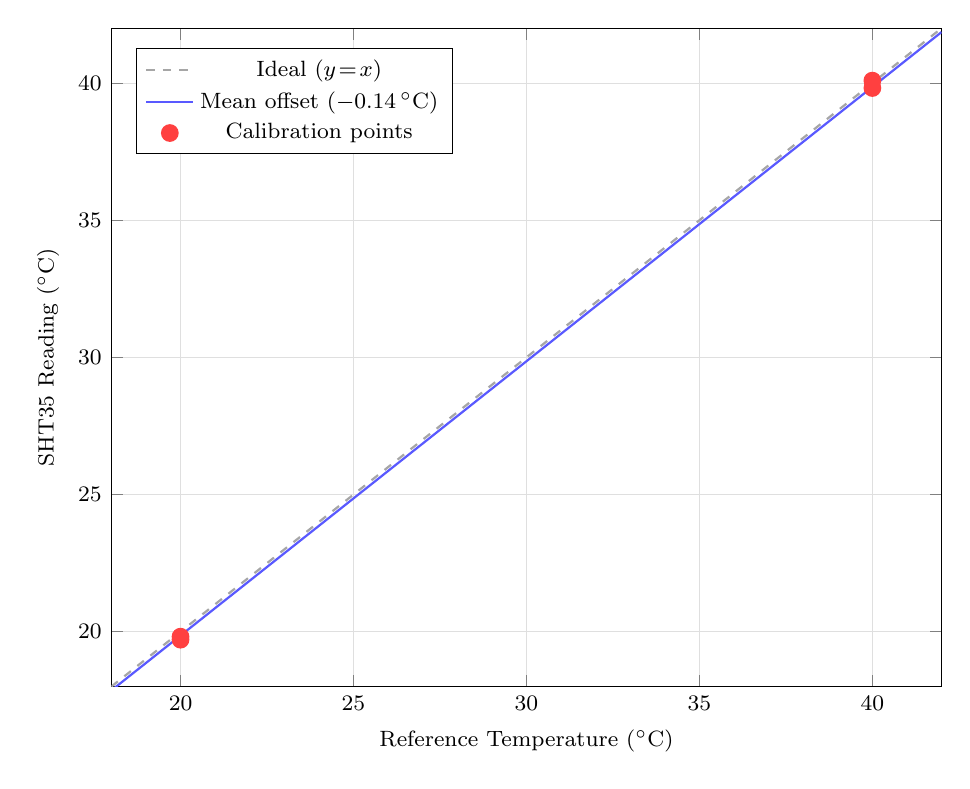
\begin{tikzpicture}
\begin{axis}[
    width=\textwidth,
    height=0.82\textwidth,
    xlabel={Reference Temperature ($^\circ$C)},
    ylabel={SHT35 Reading ($^\circ$C)},
    xmin=18, xmax=42,
    ymin=18, ymax=42,
    xtick={20,25,30,35,40},
    ytick={20,25,30,35,40},
    grid=both,
    grid style={line width=0.2pt, draw=gray!25},
    legend pos=north west,
    legend style={font=\footnotesize},
    tick label style={font=\footnotesize},
    label style={font=\footnotesize},
]
\addplot[domain=18:42, dashed, gray!70, thick] {x};
\addlegendentry{Ideal ($y\!=\!x$)}
\addplot[domain=18:42, blue!65, thick] {x - 0.14};
\addlegendentry{Mean offset ($-0.14\,^\circ$C)}
\addplot[only marks, mark=*, mark size=2.8pt, red!75, thick] coordinates {
    (20.0, 19.82) (20.0, 19.71) (40.0, 39.82) (40.0, 40.09)
};
\addlegendentry{Calibration points}
\end{axis}
\end{tikzpicture}
\caption{Temperature: consistent offset of $-0.14\,^\circ$C.}
\label{fig:sht35-temp-scatter}
\end{subfigure}
\hfill
\begin{subfigure}[b]{0.48\textwidth}
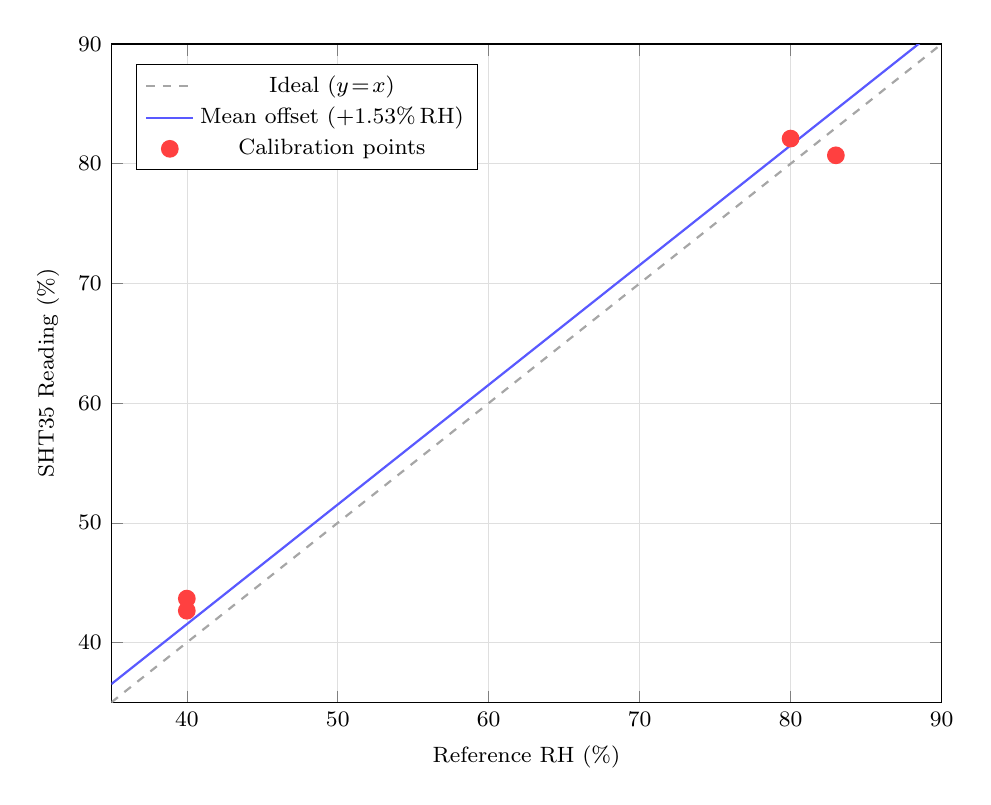
\begin{tikzpicture}
\begin{axis}[
    width=\textwidth,
    height=0.82\textwidth,
    xlabel={Reference RH (\%)},
    ylabel={SHT35 Reading (\%)},
    xmin=35, xmax=90,
    ymin=35, ymax=90,
    xtick={40,50,60,70,80,90},
    ytick={40,50,60,70,80,90},
    grid=both,
    grid style={line width=0.2pt, draw=gray!25},
    legend pos=north west,
    legend style={font=\footnotesize},
    tick label style={font=\footnotesize},
    label style={font=\footnotesize},
]
\addplot[domain=35:90, dashed, gray!70, thick] {x};
\addlegendentry{Ideal ($y\!=\!x$)}
\addplot[domain=35:90, blue!65, thick] {x + 1.53};
\addlegendentry{Mean offset ($+1.53$\%\,RH)}
\addplot[only marks, mark=*, mark size=2.8pt, red!75, thick] coordinates {
    (40.0, 43.67) (83.0, 80.70) (40.0, 42.66) (80.0, 82.10)
};
\addlegendentry{Calibration points}
\end{axis}
\end{tikzpicture}
\caption{Humidity: mean offset of $+1.53$\%\,RH with spread.}
\label{fig:sht35-humidity-scatter}
\end{subfigure}
\caption[SHT35 Calibration Scatter Plot]{SHT35 sensor readings put against the climatic chamber reference at the four calibration setpoints. The dashed diagonal represents what the perfect agreement would look like and the solid blue line is the fitted mean offset. Temperature behaviour is linear and consistent because all of the points fall within $\pm$0.3$^\circ$C of the offset line. The humidity points however show an increased residual spread across the range from $+3.67$\% at 40\%\,RH to $-2.30$\% at 83\%\,RH which indicates non-linearity that the single global correction ($-1.53$\%\,RH) doesn't fully capture.}
\label{fig:sht35-calibration-scatter}
\end{figure}

\clearpage
\subsection{Spectral sensor calibration}
\label{sec:tcs3448-calibration}

The TCS3448 spectral sensor was calibrated against a CM110 monochromator \parencite{oceanhood-monochromator} (the wavelength source) and combined with a reference power meter. The monochromator (Figure \ref{fig:monochromator-setup}) isolates a narrow-band wavelength from a broadband source and directs it toward the sensor, while the power meter provides a traceable irradiance reference at each wavelength step.

\begin{figure}[H]
    \centering
    \begin{subfigure}[b]{0.45\textwidth}
        \centering
        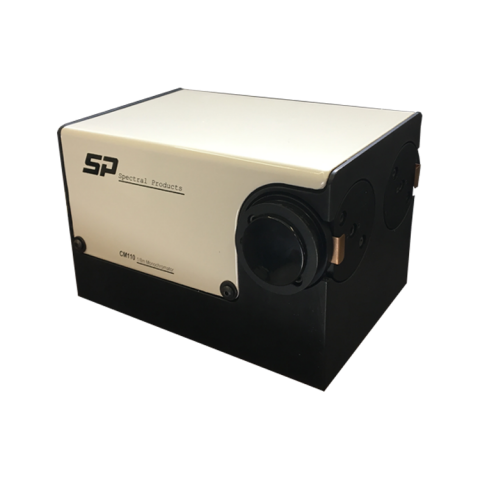
\includegraphics[width=\textwidth]{Images/monochromator_cm110}
        \caption{Oceanhood CM110 Monochromator.}
        \label{fig:monochromator}
    \end{subfigure}
    \hfill
    \begin{subfigure}[b]{0.45\textwidth}
        \centering
        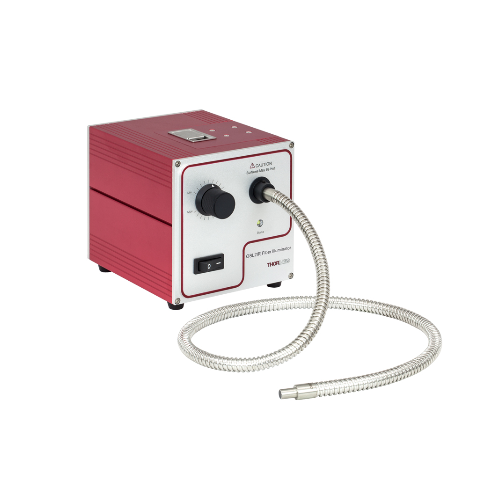
\includegraphics[width=\textwidth]{Images/light_source}
        \caption{Stabilized broadband light source.}
        \label{fig:light-source}
    \end{subfigure}
    
    \vspace{0.5em}
    \begin{subfigure}[b]{0.45\textwidth}
        \centering
        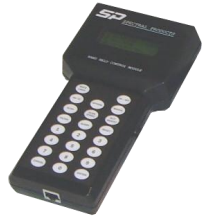
\includegraphics[width=\textwidth]{Images/CM1210}
        \caption{CM1210 Monochromator Controller.}
        \label{fig:cm1210-controller}
    \end{subfigure}
    \hfill
    \begin{subfigure}[b]{0.45\textwidth}
        \centering
        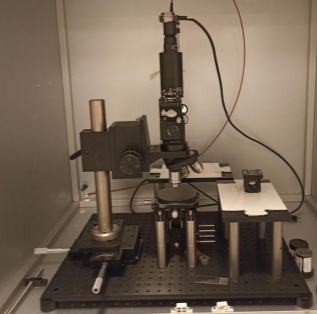
\includegraphics[width=\textwidth]{Images/optosetup}
        \caption{Full optical calibration bench setup.}
        \label{fig:opto-setup}
    \end{subfigure}
    \caption[Spectral Calibration Setup at the WELCOME Lab]{The spectral calibration setup at the WELCOME lab, including the monochromator for wavelength isolation, the power meter, the stabilized light source and the test bench configuration \parencite{oceanhood-monochromator, welcome-lab}.}
    \label{fig:monochromator-setup}
\end{figure}

The sweep ran from 300\,nm to 940\,nm in 20\,nm steps. It needed two diffraction gratings as per the test bench configuration. Grating~1 (2400\,G/mm, blaze 240\,nm) handled 300--680\,nm, and Grating~2 (1200\,G/mm, blaze 750\,nm) handled 600--940\,nm. A grating fans broadband light out into its separate wavelengths. The groove density sets how finely it resolves them, and the blaze angle tilts the diffraction efficiency toward a peak at the design wavelength, which is what keeps the signal-to-noise ratio high across the sweep. At each step I logged the monochromator output power on the reference power meter and, at the time, read the TCS3448 raw counts from the RPi API using the simple script.

The sweep showed that the empirical peak wavelengths of the visible TCS3448 channels (F1--F7) sit consistently below the typical values listed in the manufacturer datasheet \parencite{ams-osram-tcs3448}, by about 25\,nm on average (individual channels range from $\sim$16\,nm to $\sim$37\,nm). The empirical peaks of F8 (datasheet typical 748\,nm) and NIR (datasheet typical 855\,nm) fall well within the 20\,nm resolution of the sweep of their datasheet values, showing no comparable offset. Two non-exclusive mechanisms can explain the visible-channel offset. The first is a normal sensor property which is the manufacturing-lot variation. The second is a that a near-uniform offset across all visible channels also indicates a small systematic wavelength-calibration offset in the monochromator itself. The current single benchmarking data cannot fully separate the two causes. Resolving this issue would demand an independent wavelength reference such as a calibrated spectral line source, identified as future work in Section~\ref{sec:future-work}. For the platform's current single-station use the practical impact is limited: the offset is consistent and repeatable, so within a given station the channel ordering and the relative spectral structure are preserved (Figure~\ref{fig:tcs3448-comparison}). The distinction is not irrelevant, however, for \emph{absolute} wavelength labelling: if the shift originates in the monochromator rather than the sensor, the sensor's true peaks remain near the datasheet values and the empirical mapping would mislabel them by about 25\,nm. Settling this requires an independent wavelength reference or a per-station sweep, both identified as future work in Section~\ref{sec:future-work}. With that caveat, the offset is encompassed by the empirical channel mapping, derived from the wavelengths where each channel showed its maximum response. This is summarized in Table~\ref{tab:tcs3448-channel-mapping} and used throughout the platform.

\begin{figure}[H]
    \centering
    \begin{subfigure}[b]{0.48\textwidth}
        \centering
        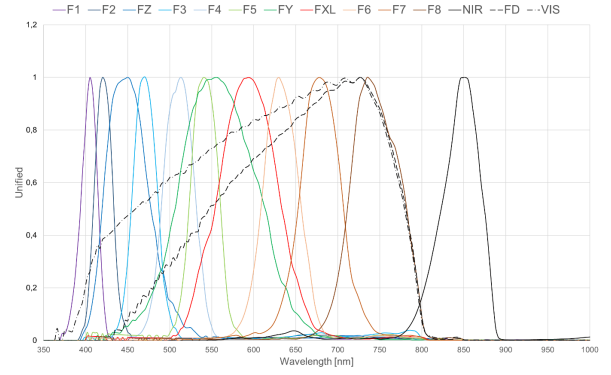
\includegraphics[width=\textwidth]{Images/tcs3448wavelengths}
        \caption{Theoretical responsivity. \textcopyright\ ams-OSRAM AG, reproduced from the TCS3448 datasheet for academic comparison \parencite{ams-osram-tcs3448}.}
        \label{fig:tcs3448-datasheet-wavelengths}
    \end{subfigure}
    \hfill
    \begin{subfigure}[b]{0.48\textwidth}
    \centering
    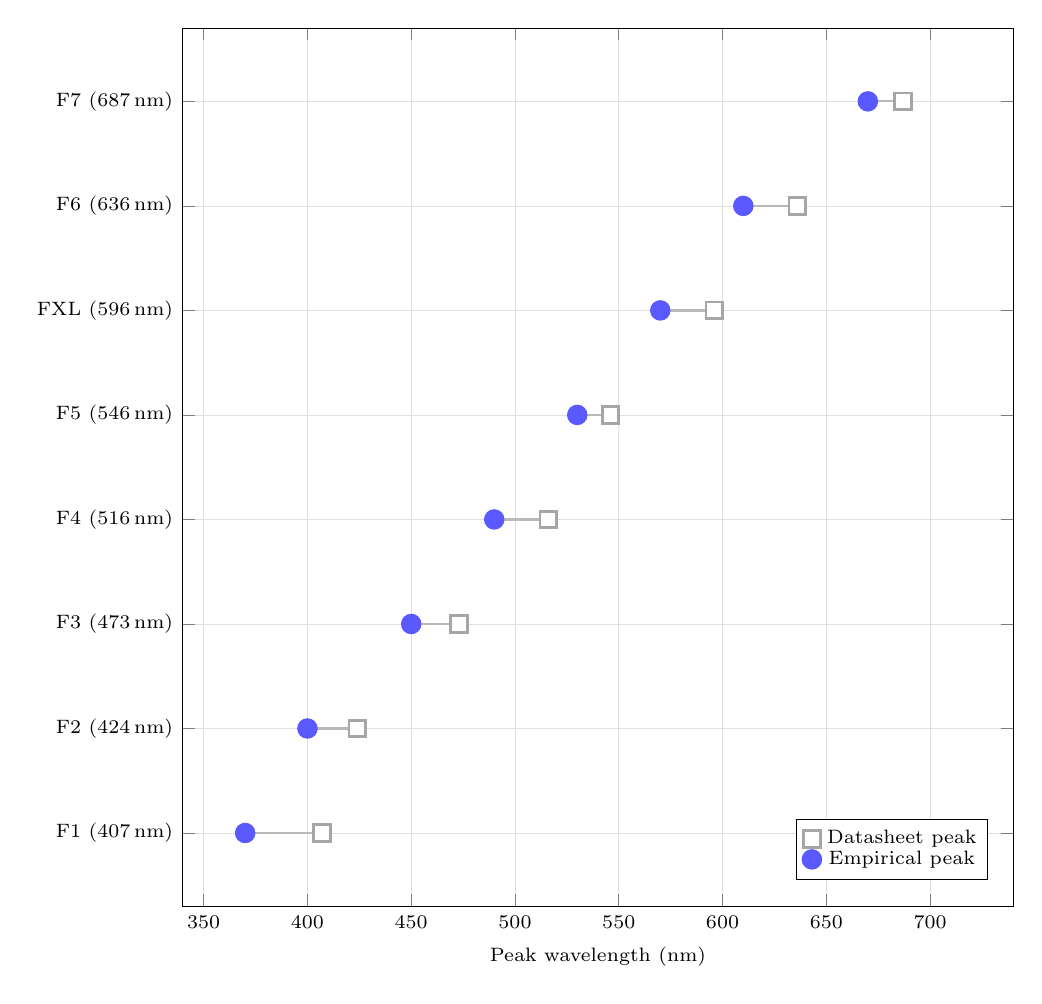
\begin{tikzpicture}
    \begin{axis}[
        width=\textwidth,
        height=1.05\textwidth,
        xlabel={Peak wavelength (nm)},
        xmin=340, xmax=740,
        ymin=0.3, ymax=8.7,
        xtick={350,400,450,500,550,600,650,700},
        ytick={1,2,3,4,5,6,7,8},
        yticklabels={%
            F1 (407\,nm),
            F2 (424\,nm),
            F3 (473\,nm),
            F4 (516\,nm),
            F5 (546\,nm),
            FXL (596\,nm),
            F6 (636\,nm),
            F7 (687\,nm)},
        grid=both,
        grid style={line width=0.2pt, draw=gray!25},
        tick label style={font=\scriptsize},
        label style={font=\scriptsize},
        legend pos=south east,
        legend style={font=\scriptsize, inner sep=2pt, row sep=-3pt},
    ]
    % Connecting lines (shift arrows)
    \addplot[gray!55, thick, forget plot] coordinates {(370,1)(407,1)};
    \addplot[gray!55, thick, forget plot] coordinates {(400,2)(424,2)};
    \addplot[gray!55, thick, forget plot] coordinates {(450,3)(473,3)};
    \addplot[gray!55, thick, forget plot] coordinates {(490,4)(516,4)};
    \addplot[gray!55, thick, forget plot] coordinates {(530,5)(546,5)};
    \addplot[gray!55, thick, forget plot] coordinates {(570,6)(596,6)};
    \addplot[gray!55, thick, forget plot] coordinates {(610,7)(636,7)};
    \addplot[gray!55, thick, forget plot] coordinates {(670,8)(687,8)};
    % Datasheet peaks (hollow squares)
    \addplot[only marks, mark=square*, mark size=3pt,
             mark options={fill=white, draw=gray!70, line width=1pt}] coordinates {
        (407,1)(424,2)(473,3)(516,4)(546,5)(596,6)(636,7)(687,8)
    };
    \addlegendentry{Datasheet peak}
    % Empirical peaks (filled circles)
    \addplot[only marks, mark=*, mark size=3.5pt, blue!65] coordinates {
        (370,1)(400,2)(450,3)(490,4)(530,5)(570,6)(610,7)(670,8)
    };
    \addlegendentry{Empirical peak}
    \end{axis}
    \end{tikzpicture}
        \caption{Empirical peak wavelengths from the monochromator sweep vs.\ the datasheet's nominal values. Each row shows one channel where the circle is what's the measured empirical peak and the square is what's the datasheet value. The horizontal gap is the shift of the visible channels. They range from $\sim$16\,nm (F5) to $\sim$37\,nm (F1), with a mean of about 25\,nm. F8 and NIR are not displayed because they aligned with their datasheet peaks within the sweep resolution.}
        \label{fig:tcs3448-empirical-response}
    \end{subfigure}
    \caption[TCS3448 Spectral Channel Peak Wavelengths: Datasheet vs.\ Empirical]{Comparison between nominal peak wavelengths from the TCS3448 datasheet and the empirical peaks determined by the monochromator sweep.}
    \label{fig:tcs3448-comparison}
\end{figure}

\clearpage
\begin{table}[htbp]
\centering
\caption[TCS3448 Empirical Channel Peak Wavelengths]{Empirical peak wavelengths of the TCS3448 channels measured by the monochromator sweep. The ``Empirical peak'' column reflects the wavelength range at which the channel registered its highest raw count during the sweep (Grating~1 was used for channels peaking below 680\,nm, and Grating~2 for channels peaking above 680\,nm).}
\label{tab:tcs3448-channel-mapping}
\small
\setlength{\tabcolsep}{5pt}
\renewcommand{\arraystretch}{1.25}
\begin{tabularx}{\textwidth}{|P{1.5cm}|X|X|P{4.5cm}|}
\hline
\textbf{Channel} & \textbf{Datasheet peak (nm)} & \textbf{Empirical peak (nm)} & \textbf{Dominant response range} \\
\hline
F1 & 407 & $\sim$360--380 & UV/Violet \\
\hline
F2 & 424 & $\sim$400 & Violet \\
\hline
F3 & 473 & $\sim$440--460 & Blue \\
\hline
F4 & 516 & $\sim$480--500 & Cyan/Green \\
\hline
F5 & 546 & $\sim$520--540 & Green \\
\hline
FXL & 596 & $\sim$560--580 & Yellow/Orange \\
\hline
F6 & 636 & $\sim$600--620 & Orange/Red \\
\hline
F7 & 687 & $\sim$660--680 & Red \\
\hline
F8 & 748 & $\sim$720--760 & Far Red / NIR edge \\
\hline
NIR & 855 & $\sim$840--900 & Near-Infrared \\
\hline
\end{tabularx}

\vspace{0.4em}
\end{table}

The complete calibration state applied to the physical station is stored in \texttt{config.ini}. Table~\ref{tab:tcs3448-calibration-state} lists the values as deployed in each station.

\begin{table}[H]
\centering
\caption[TCS3448 Deployed Calibration State]{Deployed TCS3448 calibration state as stored in \texttt{config.ini} on the station. Scale factor converts raw ADC counts to calibrated irradiance (mW/m$^2$) after dark subtraction. The dark offset is the residual count observed with the sensor fully covered.}
\label{tab:tcs3448-calibration-state}
\small
\setlength{\tabcolsep}{5pt}
\renewcommand{\arraystretch}{1.2}
\begin{tabularx}{\textwidth}{|P{1.6cm}|X|X|P{4.5cm}|}
\hline
\textbf{Channel} & \textbf{Scale factor} & \textbf{Dark offset (counts)} & \textbf{Empirical peak (nm)} \\
\hline
F1   & 0.880 & 0 & $\sim$360--380 \\
\hline
F2   & 0.864 & 0 & $\sim$400 \\
\hline
F3   & 1.063 & 0 & $\sim$440--460 \\
\hline
F4   & 1.085 & 0 & $\sim$480--500 \\
\hline
F5   & 2.90  & 0 & $\sim$520--540 \\
\hline
F6   & 9.81  & 1 & $\sim$600--620 \\
\hline
F7   & 9.68  & 2 & $\sim$660--680 \\
\hline
F8   & 9.21  & 2 & $\sim$720--760 \\
\hline
FZ   & 0.96  & 0 & Broad (CIE Z tristimulus) \\
\hline
FY   & 2.0   & 0 & Broad (CIE Y / luminance) \\
\hline
FXL  & 2.36  & 0 & $\sim$560--580 (empirical) \\
\hline
NIR  & 11.54 & 4 & $\sim$840--900 \\
\hline
\texttt{2x\_vis\_1} & 1.0 (uncal.) & 2 & Broadband visible \\
\hline
\texttt{fd\_1}      & 1.0 (uncal.) & 79 & AC-coupled (flicker) \\
\hline
\end{tabularx}
\end{table}

From the sweep data (Table~\ref{tab:tcs3448-sweep-excerpt}), a per-channel scaling factor was computed by combining the power-to-count ratio from the sweep with a normalization to spectral irradiance:
\begin{equation}
    s_k = \frac{P_{\text{ref},k}}{C_{\text{peak},k}} \cdot \frac{10^{-3}}{A_{\text{eff}}}
    \label{eq:tcs-scale}
\end{equation}
where $P_{\text{ref},k}$ [$\mu$W] is the optical power measured by the reference power meter at the wavelength of peak response for channel $k$, $C_{\text{peak},k}$ is the corresponding peak ADC count from the calibration sweep, and $A_{\text{eff}} \approx 7.0 \times 10^{-8}$\,m$^2$ is the effective per-channel optical aperture area according to the TCS3448 datasheet \parencite{ams-osram-tcs3448}. The $10^{-3}$ factor is what converts µW to mW. These factors convert raw ADC counts directly into spectral irradiance in mW/m$^2$, a range (typically 10--5000\,$\text{mW/m}^2$ per channel under indoor lighting) that is human-readable on the dashboard and matches the conventions used for photosynthetically active radiation (PAR) measurements.

\begin{table}[H]
\centering
\caption[TCS3448 Grating 1 Sweep Results (Excerpt)]{Sweep results on Grating~1 for selected channels. For each monochromator wavelength, the power meter reference and the dominant TCS3448 channel response are shown. Channels not listed peaked below the noise floor at the given wavelength.}
\label{tab:tcs3448-sweep-excerpt}
\small
\setlength{\tabcolsep}{4pt}
\renewcommand{\arraystretch}{1.2}
\begin{tabularx}{\textwidth}{|P{1.8cm}|X|X|X|}
\hline
\textbf{$\lambda$ (nm)} & \textbf{Ref. power} & \textbf{Peak channel} & \textbf{Peak counts} \\
\hline
380 & 0.333\,$\mu$W & F1 & 5\,404 \\
\hline
400 & 0.471\,$\mu$W & F2 & 7\,781 \\
\hline
440 & 0.826\,$\mu$W & F3 & 10\,121 \\
\hline
480 & 1.220\,$\mu$W & F4 & 14\,184 \\
\hline
500 & 1.319\,$\mu$W & F4 & 17\,364 \\
\hline
520 & 1.584\,$\mu$W & F5 & 7\,782 \\
\hline
560 & 2.006\,$\mu$W & FXL & 10\,625 \\
\hline
600 & 2.222\,$\mu$W & F6 & 13\,397 \\
\hline
620 & 2.205\,$\mu$W & F6 & 24\,225 \\
\hline
640 & 2.205\,$\mu$W & F6 & 17\,677 \\
\hline
660 & $2.115\,\mu$W & F7 & 21\,720 \\
\hline
680 & $2.031\,\mu$W & F7 & 20\,502 \\
\hline
\end{tabularx}

\vspace{0.4em}
\end{table}

A second calibration step addressed the sensor's electrical noise floor. Even in complete darkness, each channel produces a small number of counts due to some noise in the silicon photodiodes. These dark counts vary by channel. Longer-wavelength channels (F7, F8, NIR) exhibit higher noise than the visible-range channels. The dark baseline was measured by physically covering the sensor and recording the residual counts. Per-channel offsets were then subtracted before the irradiance scaling is applied, so the station reports exactly zero under no-light conditions.

During the second grating sweep (Grating 2, 600--940\,nm), the grating's higher power output pushed multiple channels into the 16-bit ADC ceiling of 65\,535 counts. Those points were saturated so they were dropped from the coefficient calculation. The 600--680\,nm overlap between the two gratings is used as a sanity check. I observed that each channel that peaked at a given wavelength peaked there under both gratings which confirms the channel mapping. Because the saturated peak samples were discarded, the long-wavelength scale factors (F6--F8, NIR) were computed from the largest \emph{unsaturated} counts available rather than from the true peak counts; this is why their factors in Table~\ref{tab:tcs3448-calibration-state} are several times larger than the visible-channel factors and cannot be reproduced directly from the unsaturated Grating~1 counts shown in the excerpt of Table~\ref{tab:tcs3448-sweep-excerpt}.

Everything the calibration produces is in \texttt{config.ini}. Recalibrating, if need be, only requires editing one flat file and restarting the service, with no code changes at all.

The same precision to accuracy split observed on the SHT35 shows up again here. The TCS3448 channels are precise and under steady light their responses are consistent and repeatable. The systematic wavelength shift is an accuracy problem, there's a fixed gap between where each channel is supposed to peak and where it actually does. The empirical channel mapping and the per-channel scaling factors from the monochromator sweep cancel that gap, so accuracy is restored without touching the sensor's underlying precision.

\paragraph{Measurement uncertainty.}
The 20\,nm sweep increments restrict each channel's peak wavelength to about $\pm10\,$nm. This uncertainty is fine for the broad visible channels (F1--F7) but becomes less ideal for the narrower long-wavelength ones (F8, NIR). The power meter's own accuracy rating also contributes to the scaling-factor uncertainty.

\clearpage
\subsection{Scale and camera calibration}

The load cell and HX711 ADC were carried over from \textcite{colinet2025}, who already showed they are adequate for evapotranspiration tracking on PhenoHive, so I ran no full lab sweep on them. The inherited two-point procedure is the right amount of effort for a teaching station. The tare value, the zero-load ADC reading, is taken with an empty platform, and the calibration factor comes from one known mass placed on the scale. Both numbers go into \texttt{config.ini} and are applied at read time. A dashboard wizard on the DebugUI webpage steps the TA through the two actions, which cuts down on slip-ups during deployment.

The platform now reports the plant's growth in real-world units instead of just a plain pixel count which is hard to interpret. For correct calibration, the TA sets a \texttt{pixel\_to\_cm\_ratio} through a semi-automated step where an object of known size sits in the field of view. The system then applies that ratio to its skeleton-length figure which means that students can read growth in centimeters. The station can also capture a background image on demand which gives it a clean reference for shadow removal and background subtraction that sharpens the morphological measurements. This was retained from the previous version of the platform, but the calibration step was made more user-friendly by integrating it into the DebugUI.

\section{Data gathering and signal processing}

PhenoHive has to turn physical measurements into biological indicators a student can trust. This means that data quality is the whole point here. If there's too much noise, the students start doubting the readings instead of studying plant physiology. My work therefore went into two things. First, a standard way to integrate sensors and second, a two-stage MAD filter pipeline that cleans and aggregates the raw signals before they reach storage and visualization.

\subsection{Data smoothing and noise rejection}
\label{sec:data-smoothing}

Raw sensor data can contain sudden spikes from electrical interference, I$^2$C bus jitter or physical disturbances to the scale. The pipeline applies Median Absolute Deviation (MAD) filtering \parencite{leys2013mad} at two stages to reject outliers before they reach the stored record. For a set of $n$ values, the filter computes the median $\tilde{x}$ and discards any value that satisfies the condition:
\begin{equation}
    |x_i - \tilde{x}| > k \cdot \text{MAD}, \qquad \text{where } \text{MAD} = \text{median}(|x_i - \tilde{x}|)
\end{equation}
with sensitivity factor $k = 3$ by default (configurable). At least three samples are needed for meaningful outlier detection.

\textbf{Stage~1 — burst-level.} A sensor is read $n$ times within one collection event and those reads are filtered even before they become a collection record (Figure~\ref{fig:burst-pipeline}). This allows for fine-grained spike rejection in noisy deployments.

\textbf{Stage~2 — cross-collection.} At the close of each publish window, the five records that were gathered over 600\,s all pass through the same MAD filter and are then averaged into the one single record that's then persisted locally and forwarded to InfluxDB (Figure~\ref{fig:two-tier-timing}). 

\begin{figure}[H]
\centering
\begin{tikzpicture}[
    node distance=0.5cm and 0.7cm,
    stage/.style={draw, rounded corners, align=center, text width=2.7cm,
        minimum height=0.95cm, font=\footnotesize, fill=white},
    arrow/.style={-{Latex[length=2.5mm]}, thick},
    redarrow/.style={-{Latex[length=2mm]}, dashed, red!65, thick}
]
\node[stage, fill=blue!8]    (burst) {$n$ raw reads\\(burst window)};
\node[stage, fill=yellow!10, right=of burst]  (plaus) {Plausibility\\guard\\(physical limits)};
\node[stage, fill=orange!10, right=of plaus]  (mad)   {MAD outlier\\rejection\\($|x_i-\tilde{x}|>k\!\cdot\!\mathrm{MAD}$)};
\node[stage, fill=green!8,   right=of mad]    (agg)   {Aggregate\\survivors\\($\bar{x}$, $\sigma$, min, max)};
\node[stage, fill=green!15, draw=green!50, right=of agg] (pub) {Published\\record +\\quality flags};

\draw[arrow] (burst) -- (plaus);
\draw[arrow] (plaus) -- (mad);
\draw[arrow] (mad)   -- (agg);
\draw[arrow] (agg)   -- (pub);

\draw[redarrow] (plaus.south) -- ++(0,-0.65)
    node[below, font=\tiny, red!70] {discard};
\draw[redarrow] (mad.south)   -- ++(0,-0.65)
    node[below, font=\tiny, red!70] {discard + log};
\end{tikzpicture}
\caption[Burst Sampling and Signal Processing Pipeline]{Per-collection signal processing pipeline. Each collection event makes $n$ raw sensor reads where the values that are outside of physical plausibility bounds are immediately discarded. The MAD filter then removes each statistical outlier from the remaining burst. This means that the surviving samples are all aggregated into one smoothed value with quality metadata appended for storage and display.}
\label{fig:burst-pipeline}
\end{figure}

Figure~\ref{fig:mad-filtering} shows the cleaning effect on a real temperature trace. Before the MAD filtering stage, the plausibility guards throw out physically impossible values, such as humidity outside 0--100\,\% or negative illuminance, and logs them as invalid readings.

\begin{figure}[H]
    \centering
    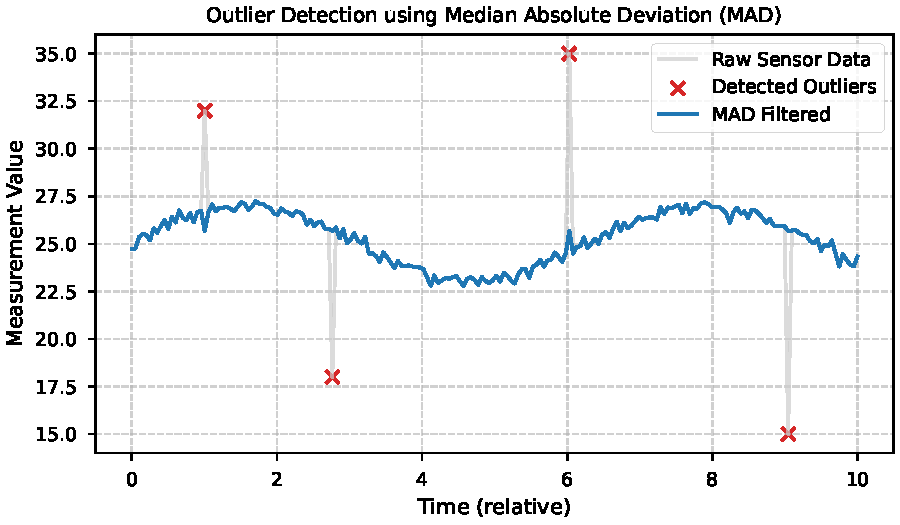
\includegraphics[width=0.85\textwidth]{Images/mad_filtering}
    \caption[Signal Cleaning Using MAD Filtering]{Signal cleaning using Median Absolute Deviation (MAD). This two-stage pipeline identifies and removes anytransient spikes that are caused by electrical interference or physical disturbances. This prevents them from corrupting any long-term trend analysis.}
    \label{fig:mad-filtering}
\end{figure}

\subsection{Confidence flags and quality metadata}

When publishing the aggregated record, the system does not only output a single smoothed value. It also includes statistical indicators of the signal's stability over the window, such as the minimum, maximum and standard deviation.
Each sensor reading is also tagged with confidence metadata. The system tracks the ratio of successful reads to attempted reads and computes the coefficient of variation (CV) within the burst:
\begin{equation}
    CV = \frac{\sigma}{\mu}
\end{equation}
where the sample mean $\mu$ and sample standard deviation $\sigma$ are calculated by the acquisition pipeline from the set of valid, post-filtering samples collected during the burst window. If the success ratio goes below a configured threshold or the $CV$ exceeds the maximum allowed variation, the record is then flagged with a \texttt{low\_confidence} marker.

\subsection{Acquisition summary}

Taken together, the acquisition layer pulls back from a hardware-first view. It hides the hardware specifics, filters out physical noise, and holds every channel to a calibration that traces back to laboratory references.

After calibration, the temperature reading is verified to agree with the reference chamber to within its $\pm$0.3$^\circ$C setpoint tolerance, with the SHT35's own datasheet accuracy ($\pm$0.1$^\circ$C) remaining the limiting figure. The humidity measurement holds around $\pm$2.2\,\% RH across the usual 40--80\,\% indoor range. The Spectral channels now are now mapped to physical irradiance units with per-channel dark subtraction. This means that what reaches the student is data they is ready to be read and interpreted biologically.

